%% This is a semi-simple sample document.

\documentclass{article} % \documentclass{} is the first command in any LaTeX code.  It is used to define what kind of document you are creating such as an article or a book, and begins the document preamble

%\usepackage[spanish]{babel} % Para traducir palabras claves al español como "Figure" -> "Figura"

\usepackage{amsmath, amssymb} % \usepackage is a command that allows you to add functionality to your LaTeX code

\usepackage{mathtools} % using cases inside equations

\usepackage{graphicx} % image package

\usepackage{float} % Float specifiers are written in the square brackets whenever we use a float such as a figure or a table

\usepackage{subcaption} % more than one picture s in the same figure

\parskip 0.1in %paragraph distance

\usepackage[margin=0.984252in]{geometry} %margin

\usepackage[hidelinks]{hyperref} % Magic for index linking

\usepackage{chngcntr} % For figure number matching with section number
\counterwithin{figure}{section}

\usepackage{appendix} % Appendix

\usepackage{listings} % Para display codigo

\usepackage{enumitem} % para enuimerar empezando por a, b, c

\usepackage{listings} % para meter codigo

\title{Trabajo Práctico N°2} % Sets article title
\date{Septiembre 2023} % Sets article date

\author{
	\textbf{Fundamentos de Análisis de Datos}\\
	Maestría en Ciencia de Datos\\
	\\~\\
	\textbf{Estudiantes: }\\
	\textbf{Ing. Flores, Matías Gabriel}\\
	matflores@itba.edu.ar
 	\\~\\
 	\textbf{Ing. Loiseau, Matías}\\
 	mloiseau@itba.edu.ar
 	\\~\\
	\textbf{Docente: }\\
	\textbf{Dra. Rey, Andrea A.}
}

% The preamble ends with the command \begin{document}
\begin{document} % All begin commands must be paired with an end command somewhere

\begin{figure}
\centering
	
\includegraphics[width=0.2\textwidth]{images/itba-logo}
	%\caption{Mi Figure}
	\label{fig:itba-logo}
\end{figure}
\maketitle % creates title using information in preamble (title, author, date)

\thispagestyle{empty} % Ignore page number
\cleardoublepage

\cleardoublepage
\tableofcontents % general index
\cleardoublepage


\section{Ejercicio N° 1}

Vamos a trabajar con el archivo \textit{MedidasCorporales.xlsx}.

\subsection{Primer punto}

\textbf{Consigna:} ¿Cuántos registros y cuántas variables tiene el conjunto de datos? ¿Todas las variables
son numéricas?

El set de datos de Medias Corporales tiene 507 registros y 24 variables. Verificamos que no haya nulos. Esto se puede visualizar en la tabla \ref{tab:table-punto-1-1}. Además, durante el análisis de los datos pudimos verificar que todas las variables son numéricas.

\begin{table}[H]
	\centering
		\begin{tabular}{||l | c ||}
			\hline
			\hline
			 & Valor\\
			\hline			
			\hline
			Registros & 507\\
			\hline
			Columnas & 24\\
			\hline
			Nulos & 0 \\
			\hline
			\hline
		\end{tabular}
		\caption{Cantidad de campos en el set de datos.}
	\label{tab:table-punto-1-1}
\end{table}


\subsection{Segundo punto}

\textbf{Consigna:} Regresión lineal simple: ¿cómo influye la altura en el peso?

\begin{enumerate}[label=(\alph*)]
\item Realizar una regresión lineal simple y escribir el modelo teórico resultante.
\item ¿Cuáles son las estimaciones de la ordenada al origen y de la pendiente? ¿Son estos coeficientes de regresión significativos?
\item Calcular el error estándar residual, el coeficiente de determinación R2 y su valor ajustado. ¿Qué se podría concluir sobre la bondad de ajuste del modelo?
\end{enumerate}

Teniendo en cuenta la consigna, en primer lugar analizamos como se distribuye la variable de peso en función a la de altura mediante un diagrama de dispersión, figura \ref{fig:scatter1}. 


\begin{figure}[H]
	\centering
	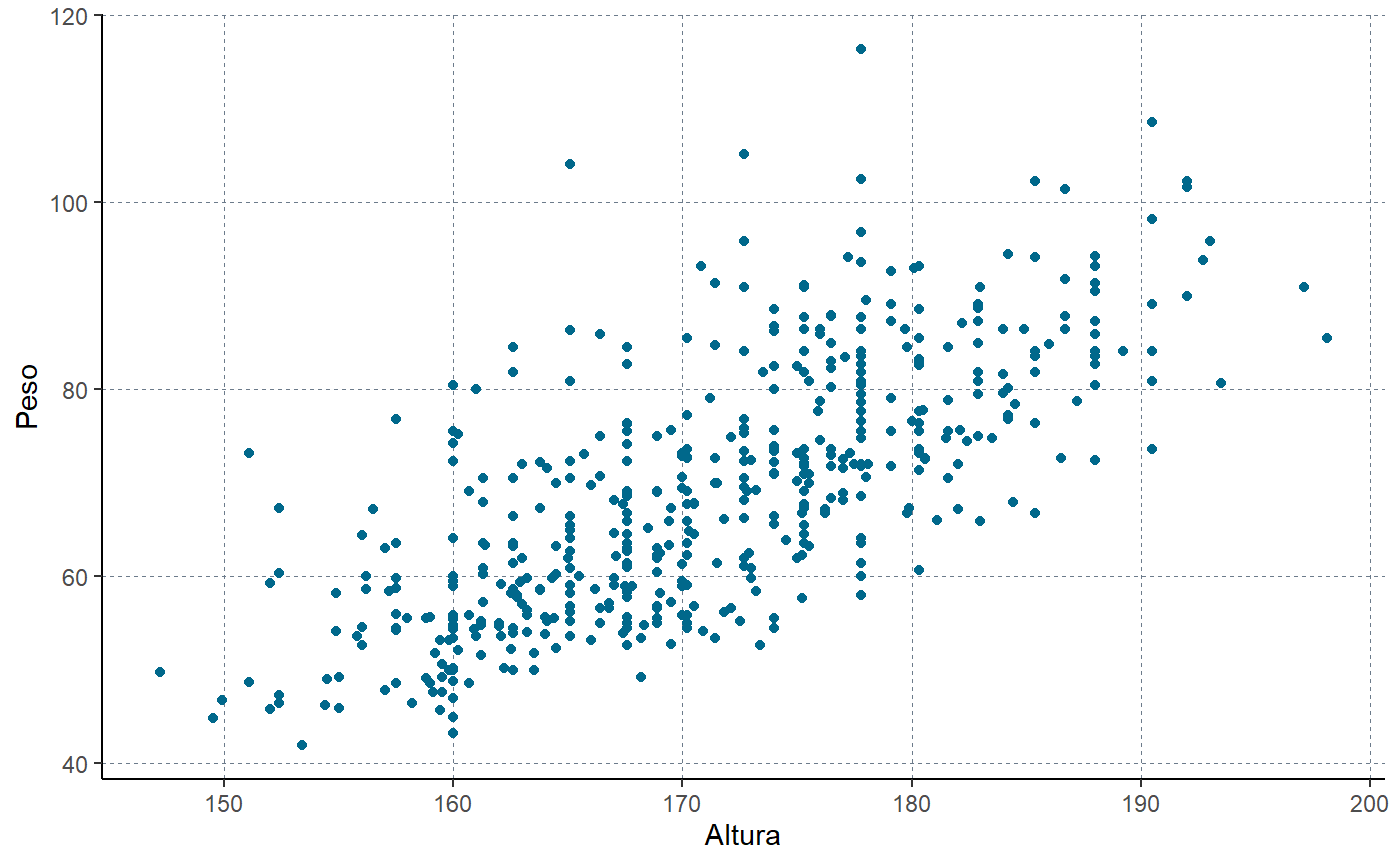
\includegraphics[width=0.8\textwidth]{images/1-2 Scatter}
	\caption{Diagrama de dispersión entre Peso y Altura.}
	\label{fig:scatter1}
\end{figure}

Analizando el gráfico obtenido, podemos ver que pareciera haber una correlación positiva entre ambas variables. Realizando el calculo de correlación obtenemos como resultado un valor de 0.717, por lo tanto podemos determinar que se encuentran bastante correlacionadas. 

Luego, procedimos a realizar el modelo de regresion lineal, teniendo como variable dependiente al peso, y variable independiente a la altura. Como resultado, el modelo teórico queda de la siguiente forma:


\begin{equation}
\hat{y} = -105.011 + 1.018x
\end{equation}

 donde $x$ representa la altura e $\hat{y}$ representa el peso estimado por el modelo.
 
Graficando esta recta de regresión lineal sobre el diagrama de la figura \ref{fig:scatter1}, nos queda el grafico de la figura \ref{fig:scatter2}, donde podemos observar que la linea se ajusta a los puntos.

\begin{figure}[H]
	\centering
	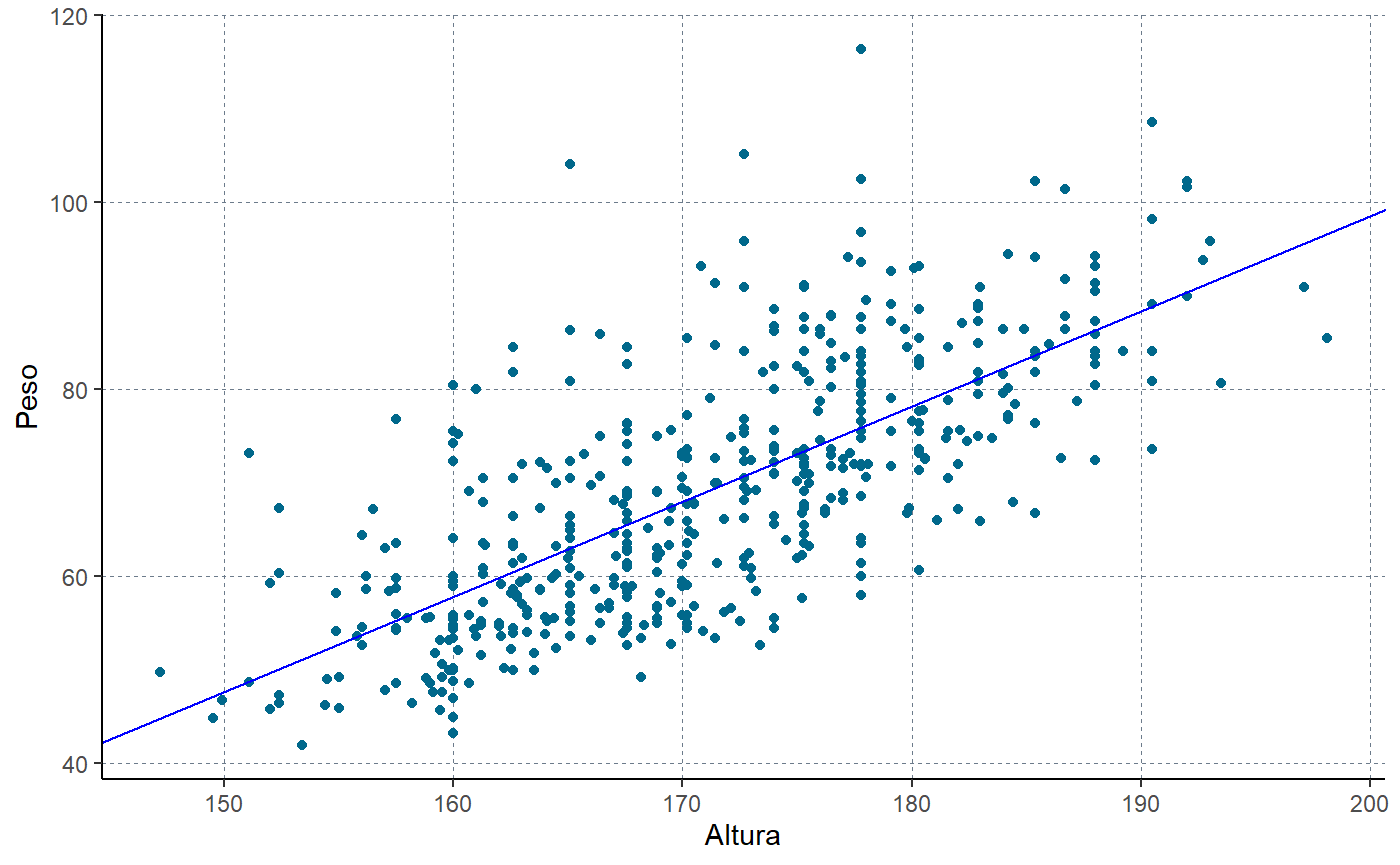
\includegraphics[width=0.8\textwidth]{images/1-2 Scatter Recta}
	\caption{Diagrama de dispersión entre Peso y Altura con Recta.}
	\label{fig:scatter2}
\end{figure}

La estimación de la ordenada al origen es $-105.011$ y de la pendiente es $1.018$. Al ser una pendiente positiva, a medida que el valor de x aumente, el de y también tenderá a aumentar. Estos coeficientes de regresión tienen un alto grado de significancia según los resultados obtenidos.

El error estándar residual resultante determina que la estimación promedio del peso puede diferir en 9.308kg. En cuanto al coeficiente de determinación $R^2$ obtenido, consideramos que es un valor significativamente moderado. Por ultimo, el valor ajustado del coeficiente nos dio bastante similar al original. Estos valores se pueden observar en la Tabla \ref{tab:table-punto-1-2-c}.

\begin{table}[H]
	\centering
		\begin{tabular}{||l | c ||}
			\hline
			\hline
			Variable & 	Valor\\
			\hline			
			\hline
			Residuo & 9.308\\
			\hline
			$R^2$ & 0.5145\\
			\hline
			Valor ajustado & 0.5136 \\
			\hline
			Estadístico-F & 354.4 \\
			\hline
			P-Valor & $<2.2e^{-16}$ \\
			\hline
			\hline
		\end{tabular}
		\caption{Parámetros de salida del modelo.}
	\label{tab:table-punto-1-2-c}
\end{table}


A partir de los resultados obtenidos, determinamos que el 51\% de las variaciones de los pesos están explicadas por la altura de las personas. Además, podemos concluir que existe una relación lineal significativa entre la altura y el peso, ya que el estadístico-f observado tiene un valor alto con un p-valor menor a $0.05$, rechazando la hipótesis nula.

\subsection{Tercer punto}

\textbf{Consigna:} Regresión lineal múltiple: ¿cómo influyen las medidas consideradas en el peso?

\begin{enumerate}[label=(\alph*)]
\item Guardar en la variable n la cantidad total de registros.
\item Fijar una semilla igual a 1234 y correr el siguiente comando:
\begin{lstlisting}
muestras <- 1:n %>%
	createDataPartition(p=0.8,list=FALSE)
\end{lstlisting}
Usar la variable muestras para separar aleatoriamente el conjunto de registros en conjuntos de entrenamiento y de prueba. ¿Qué porcentaje de los datos integra cada uno de estos conjuntos?
\item A partir del conjunto de entrenamiento, realizar el modelo de regresión lineal múltiple con todas las variables involucradas.
\item A partir del conjunto de entrenamiento, realizar el modelo de regresión lineal múltiple con las variables que presenten un nivel de confianza de al menos el 95\%.
\item Utilizando el conjunto de prueba, calcular el error cuadrático medio:
$$
MSE=\frac{1}{n}\sum^n_{i=1}(y_i-\hat{y}_i)^2
$$
donde n es la cantidad total de predicciones, $y_i$ es el valor real de la variable respuesta e $\hat{y}_i$ es el valor predicho. ¿Cuál de los dos modelos muestra un valor menor de MSE?
\end{enumerate}

Para este ejercicio, en primer lugar, dividimos el dataset en un conjunto de entrenamiento y uno de prueba, mediante la semilla y el comando establecidos. Una vez realizado esto, el set de datos de entrenamiento resultante nos quedó con un 80\%  del data set original, mientras que el de prueba con un 20\%.

Luego de haber separado el dataset, pasamos a realizar los modelos de regresión lineal multiple solicitados. En este caso, realizamos 2 modelos para ver que como influyen las variables en el peso. En el primer modelo utilizamos todas las variables del dataset, mientras que para el segundo utilizamos solo las variables que presentaran al menos un 95% de confianza. Para determinar estas variables, analizamos la confianza obtenida y procedimos a crear un nuevo modelo descartando las variables que no superaran ese porcentaje.

Al realizar el primer modelo, obtuvimos los coeficientes de regresión que se encuentran en la tabla siguiente:


TABLA


Luego, procedimos a analizar el nivel de confianza obtenido, que se encuentra en la tabla.

TABLA 2.

A partir de estos valores, determinamos las variables que utilizaríamos en el modelo 2. A partir de la confianza calculada, tomamos en cuenta todos los valores que no pasaran por cero. Por lo tanto, las variables que utilizamos fueron "Profundidad de pecho", "Diámetro de rodilla", "Contorno de pecho", "Contorno de cintura", "Contorno de cadera", "Contorno de muslo", "Contorno de antebrazo", "Contorno de rodilla", "Contorno de pantorrilla", "Edad" y "Altura". Los coeficientes obtenidos para este modelo se encuentran en la siguiente tabla.

TABLA 3

Finalmente, habiendo entrenado los dos modelos sobre el conjunto de entrenamiento, procedimos a realizar las predicciones sobre el conjunto de prueba. Una vez obtenidas las predicciones, llevamos a cabo el calculo del error cuadrático medio para cada uno. Como resultado, obtuvimos los valores que se detallan en la tabla \ref{tab:table-punto-1-3}.


\begin{table}[H]
	\centering
		\begin{tabular}{||l | c || c || c || c || c || c ||}
			\hline
			\hline
			Modelo & Residuo & $R^2$ & $R^2$ Ajustado & Estadistico F & P-Valor & MSE\\
			\hline			
			\hline
			1 & 2.077 & 0.97 & 0.97 & 710 & $<2.2e^{-16}$ & 5.630\\
			\hline
			2 & 2.098 & 0.97 & 0.97 & 1454 & $<2.2e^{-16}$ & 5.369\\
			\hline
			\hline
		\end{tabular}
		\caption{Errores cuadráticos medios.}
	\label{tab:table-punto-1-3}
\end{table}

A partir de los resultados obtenidos, podemos observar que el Estadistico F del modelo 2 tiene mas que el doble de tamaño que el del primer modelo, determinando que posee una mejor capacidad de explicar la variabilidad del peso en base a las variables involucradas. Los otros resultados dieron bastante similares para ambos, siendo el residuo levemente mas alto en el modelo 2. Por ultimo, el segundo modelo es el que presenta un menor error cuadrático medio, siendo el que tiene un mejor ajuste, y el mas eficiente de los dos.

\section{Ejercicio N° 2}

Vamos a trabajar con el archivo \textit{Dolor.xlsx}. El mismo contiene una muestra de 3504 pacientes que acudieron a un centro de salud presentando dolor en el pecho. Para estos pacientes, se recogieron diversas medidas. En el caso de las variables estrechamiento de arterias coronarias y de tres arterias coronarias, ambas son variables binarias que indican la presencia de estrechamiento en alguna de las arterias coronarias de al menos un 75\% (valor igual a 1) o no (valor igual a 0). En cuanto a la variable sexo, 0 corresponde a masculino y 1 a femenino.

\subsection{Primer punto}

\textbf{Consigna:} Realizar un modelo de regresión logística simple, que estudie la presencia de estrechamiento en alguna arteria coronaria explicada por el colesterol. Escribir la ecuación del modelo resultante y calcular la probabilidad de que una persona con un nivel de colesterol igual a 199 presente estrechamiento arterial.

En primer lugar, realizamos un analisis del dataset con el que ibamos a trabajar. Este conjunto de datos se encuentra compuesto por 7 variables numericas. Lo primero que pudimos encontrar, fue la presencia de valores nulos, por lo cual decidimos eliminarlos. Una vez realizado esto, detectamos que la variable "Colesterol", si bien estaba compuesta por valores numericos, era de tipo "Char" con campos llamados "NA", lo cual sería un conflicto al realizar el modelo. Por lo tanto, eliminamos estos valores y convertimos la variable a tipo numérica, quedando así con 2258 registros. 

Para realizar el modelo de regresión logística simple, decidimos utilizar la variable "Estrechamiento arterias coronarias" como nuestra variable dependiente, y "Colesterol" como la independiente. Mediante este modelo, obtuvimos los coeficientes necesarios para determinar la ecuación resultante. 

\begin{equation}
p(x)=\frac{\exp(-0.7525280 + 0.0062268x)}{1 + \exp(-0.7525280 + 0.0062268x)}
\end{equation}

Mediante el modelo implementado, pudimos calcular la probabilidad de que una persona con un nivel de colesterol de 199 presente estrechamiento arterial, siendo este un 61%. 

$p(199)=0.6193053$



\subsection{Segundo punto}

\textbf{Consigna:} Realizar un modelo de regresión logística múltiple, que estudie la presencia de estrechamiento en alguna arteria coronaria usando todas las variables no categóricas como variables explicativas. ¿Qué puede decirse sobre la significancia de las variables predictoras?

Las variables que tuvimos en cuenta para este punto fueron "Edad", "Días con Sintomas" y "Colesterol". Al realizar el modelo, obtuvimos los resultados que se encuentran en la tabla.

Tabla

Mediante estos resultados, podemos ver que tanto "Edad" como "Colesterol", tienen un coeficiente positivo, por lo que el aumento de estas dos variables se puede aumentar las probabilidades de tener Estrechamiento en alguna arteria coronaria, teniendo una fuerte signficancia en el modelo. Por otro lado, la cantidad de Días con Sintomas no parece tener una relación signficativa con la variable dependiente. 


\subsection{Tercer punto}

\textbf{Consigna:} Replicar el modelo anterior pero diferenciando entre mujeres y varones. ¿Existen diferencias entre las significancias de las variables explicativas en función del sexo? Justificar la respuesta.

Realizando el anterior modelo para mujeres y varones por separado, a simple vista, no parece tener un fuerte impacto en los valores obtenidos para cada uno. 

TABLA DE HOMBRES Y MUJERES COMPARATIVA.

Para el grupo de Mujeres, la variable de D[ias con Sintomas pareciera tener una mayor significancia, teniendo un p-valor cerca al 0.05, a diferencia del grupo de Hombres. Por otro lado, las otras variables parecen tener la misma significancia en ambos grupos. 


\section{Ejercicio N° 3}

Vamos a trabajar con el archivo Europa.xlsx.

\subsection{Primer punto}

\textbf{Consigna:} ¿Cuáles son las variables de interés?

Mati?

\subsection{Segundo punto}

\textbf{Consigna:} Calcular la matriz de covarianza de los datos y analizar si es inversible.

Primero realizamos la matriz de covarianzas y luego aplicamos la funcion para determinar si era inversible.

MATRIZ DE COVARIANZAS.

El resultado de la invarianza fue 1.235391e+19. Como dicho valor es distinto a 0, determinamos que es inversible.

\subsection{Tercer punto}

\textbf{Consigna:} ¿Cuál es el mayor autovalor de la matriz de covarianzas?

A partir de los autovalores obtenidos en la matriz de covarianzas, determinamos que el mayor autovalor es el de la variable "Area"

\subsection{Cuarto punto}

\textbf{Consigna:} Realizar un PCA y hallar la cantidad necesaria de componentes principales para explicar al menos el 90\% de la varianza total de los datos.

Tabla con los PC

En base a los componentes principales calculados, determinamos que con 4 componentes podemos explicar un 89.25% de la varianza total de los datos, llegando así casí un 90% de ellos.

\subsection{Quinto punto}

\textbf{Consigna:} Realizar e interpretar un gráfico que visualice la contribución de las variables en las dos primeras componentes principales.

Teniendo en cuenta las funciones realizadas en los puntos anteriores, procedemos a realizar un grafico para demostrar la contribución de las variables en las dos primeras componentes principales. 


Figura del grafico.


Pregunta para Mati... 2 primeras componentes?????

\section{Ejercicio N° 4}

Vamos a considerar el conjunto de datos JohnsonJohnson disponible en R.

\subsection{Primer punto}

\textbf{Consigna:} ¿Qué tipo de datos mide esta serie de tiempo? ¿Cuál es el período de tiempo analizado?

Esta serie de tiempo contiene las ganancias en dolares trimestrales de "Johnson y Johnson", desde el año 1960 hasta 1980.

\subsection{Segundo punto}

\textbf{Consigna:} Graficar la serie tiempo, junto con sus descomposiciones aditiva y multiplicativa. ¿Se observa tendencia? ¿Se observa estacionalidad?

Lo primero que realizamos fue el grafico de la serie de tiempo. Esta se puede ver en la figura... 

Figura 


En este grafico podemos visualizar un incremento en las ganancias a lo largo del tiempo. Para analizar la tendencia y la estacionalidad en detalle, vamos a realizar las descomposiciones aditiva y multiplicativa. 

Primero vamos a analizar la descomposición aditiva. La tendencia se puede visualizar en la figura... 

Figura... 

A partir del grafico, vemos que puede llegar a tener una tendencia positiva. Para saber con exactitud el valor de tendencia, realizamos el calculo de la fuerza de tendencia. 

INSERTESE ECUACION DE FUERZA DE TENDENCIA DEL PDF. 

Al realizar el calculo de la fuerza de tendencia nos da como resultado un 0.97. Por lo que podemos determinar que existe una fuerte tendencia positiva.

Lo siguiente que se analizó fue la estacionalidad, que se puede visualizar en la figura....



figura de estacionalidad.... 


Calculamos la fuerza de la estacionalidad mediante la siguiente ecuacion


Insertese ecuacion de estacionalidad.


Esto nos da como resultado 0.32, siendo un resultado relativamente chico.

Luego, pasamos a analizar la descomposición multiplicativa. El grafico de tendencia se puede ver en la figura.... 


figura de tendencia....

Nuevamente, parece tener una tendencia alta. Al realizar el calculo de fuerza, nos da como resultado 0.99, por lo tanto, determinamos que tiene una alta tendencia.

Finalmente, realizamos el analisis de la estacionalidad, representado en la figura ..

figura de estacionaldiad....

Nuevamente, realizando el calculo de fuerza de estacionalidad, nos da como resultado 0.55. Un valor bastante superior al 0.32 de la aditiva. 

En base al analisis realizado en este punto, podemos determinar que existe una alta tendencia en la serie de tiempo, por otro lado, los valores de estacionalidad no son significativamente altos, aunque tampoco podemos determinar que sean despreciables.

\subsection{Tercer punto}

\textbf{Consigna:} Analizar la conveniencia de aplicar la transformación de Box-Cox.

Teniendo en cuenta el analisis realizado en el punto anterior, creemos conveniente realizar una transformacion de Box-Cox sobre la serie de tiempo trabajada. Mediante esta transformación vamos a estacionar la serie de tiempo, lo cual nos va a ayudar a reducir la tendencia y estacionalidad que tiene actualmente, para mas adelante poder realizar la implementacion de un modelo ARIMA. 
Para realizar la transformación, primero vamos a realizar la busqueda del mejor parametro $\lambda$. En nuestro caso, nos dio 0.15. Teniendo este valor, procedemos a realizar la transformada. En la figura ... se puede ver la comparativa entre la serie original y la transformada.

Figura

Analizando los graficos, determinamos que conviene realizar la transofrmacion, y continuar trabajando con la transormada, en lugar de la original. 

\subsection{Cuarto punto}

\textbf{Consigna:} Usar toda la información de todos los años salvo los dos últimos para realizar un modelo ARIMA automático y uno personalizado, explicando la elección de los órdenes elegidos y teniendo en cuenta lo concluido en el punto anterior. Trabajar con  $1 \leq p \leq 14$ y $1 \leq q \leq 30$.



\subsection{Quinto punto}

\textbf{Consigna:} ¿Cuáles son los parámetros obtenidos para el modelo ARIMA automático?



\subsection{Sexto punto}

\textbf{Consigna:} Predecir las ganancias del último año utilizando los dos modelos ARIMA hallados. Calcular el criterio de información de Akaike (AIC) y el error de porcentaje medio absoluto (MAPE) en cada caso y decidir, en función de estos valores, qué modelo realiza las mejores predicciones.

Tabla con la comparacion...

\end{document} % This is the end of the document
